\documentclass{book}
\usepackage{amssymb,amsmath}
\usepackage{url}
\usepackage{listings}
\usepackage{theorem}
\usepackage{graphicx}
%\usepackage{caption}
\usepackage{subfig}
\usepackage{gb4e}
\usepackage{minitoc}
\usepackage{array}
\usepackage{framed}
\usepackage{wrapfig}
\usepackage{makeidx}
\usepackage{imakeidx}
\usepackage{blindtext}
\setlength{\emergencystretch}{2pt}
\makeindex[name=classes,title={Index of Classes}]

\makeindex
\renewcommand{\mtcSfont}{\small\normalfont}
\begin{document}

\title{The Sigma Manual \\ A Guide for Users and Developers \\ of the SUMO Toolset}
\author{Adam Pease}

\maketitle
\date

\nomtcrule
\dominitoc[n]
\setcounter{secnumdepth}{1}
\setcounter{tocdepth}{1}
\tableofcontents
\listoffigures

\chapter{Preface}

\section{Introduction}

The Suggested Upper Merged Ontology (SUMO) began as a simple project to create a
high-level taxonomic structure for computer assisted training applications, but
it quickly became more ambitious, attempting to cover any topics for any
application that addressed entities in our common-sense world, and that were
amenable to symbolic processing.  It grew to cover a wide range of
representational constructs, challenging the practical use of research in
knowledge representation and reasoning.

The development of SUMO also came to encompass tools used in its development and
application.  The Sigma system \cite{p03} began as a simple ontology browsing
aid but expanded to incorporate reasoning tools created by others, first the
Vampire theorem prover \cite{RV:AICOM-2002} and then an entire suite of
reasoners called TPTP \cite{tsp08}, especially the E theorem prover
\cite{Schulz:AICOM-2002}.  That work in turn required efforts on making
reasoning practical and efficient on such a rich knowledge base \cite{psst10}.

\begin{sloppypar}
A second line of work was in relating SUMO to linguistic data, first in
developing the links from the WordNet \cite{fellbaum1998wordnet} lexical
database \cite{np03} and then developing a natural language understanding
system, called the Controlled English to Logic Translation system (CELT) that
used those links, among much other information, to translate language to logic
\cite{pl10}.  That work has been superceded by an approach called Semantic
Rewriting, which is embodied in the SigmaNLP system, whose manual is forthcoming.
\end{sloppypar}

The Sigma Knowledge Engineering Environment is a development environment for
logical theories, specifically those that extend the Suggested Upper Merged
Ontology (SUMO).  Sigma is analogous to an Integrated Development Environment
(IDE) for programming languages like C++ or Java.  Modern and expressive
languages for the development of formal theories, such as \index{SUO-KIF}SUO-KIF
\cite{Pease2009} and \index{TPTP}TPTP \cite{Sutcliffe:JAR-2009} have a similar
degree of expressiveness, in a broad sense, to a modern programming language.
Development of SUMO is done in a text editor and Sigma provides support for
browsing, debugging and applying SUMO to applications.  Like all general-purpose
programming languages, it is too expressive to allow development in any sort of
purely visual mode.  This makes it distinct from taxonomy languages, or
description logics, in which the laguages are defined primarly by their graph
structure.

We have utilized the \index{Git}Git for collaborative ontology development
rather than implementing some additional tool for collaboration. Developers are
typically given authority over one or more ontologies, required to check in
progress at least weekly so that other developers can sync up with their
changes.  This has also resulted in a detailed public record of the development
and evolution of SUMO \cite{pb10}.

Ontology is a broad area, and there are many approaches to ontology.  The purpose
of this manual is not to teach ontology, or SUMO, so a prerequisite for starting
to work with Sigma is to read the book "Ontology: A Practical Guide", and complete
all the exercises in the book.  Otherwise, many aspects of Sigma will be
mysterious.

This manual is a prerequesite for understaning the functionality of the SigmaNLP
system, although that manual is yet to be written. My hope is that this manual
will be a "living" document, subject to frequent updating as Sigma is improved and
extended.  At the moment, Sigma has a number of components that are obsolete, or
in the process of being completed or redone.

While Sigma \cite{SigmaWeb} \cite{p03} was created to support SUMO, and that has
been its primary use during some eight years of development, that is by no means
the only theory that it can handle.  Sigma works on knowledge bases that can be
composed from various files selected by the user.  Those files can be coded in a
small number of different formal languages, including TPTP and OWL, as well as
SUO-KIF.  The Sigma user can easily work with very small theories or very large
ones by composing only the theories that are needed for the work at hand.  A
typical use of Sigma would involve loading just the upper level of SUMO and
whatever domain theory is needed for the user's chosen application area.

\begin{figure}
  \centering
  \includegraphics[width=4.5in]{pictures/SigmaOver.png}
  \caption{Major Sigma functions}
  \label{fig:SigmaOver}
\end{figure}

Tools within Sigma (Figure \ref{fig:SigmaOver}) can be broadly segmented into
several groups, (1) browsing and display, (2) analysis and debugging, (3)
inference, and (4) mapping, merging and translation.

In this manual we provide an index (starting on page \pageref{classindex})) to
all the classes mentioned, so that it can be used as a reference going beyond
what one can find in the JavaDoc for Sigma\footnote{which is online at
\url{http://www.ontologyportal.org/sigmakee-doc/}}

\chapter{Code}

\section{Hello World}

The best way to learn how to use a code library is to start doing something with it. So,
we'll start with a "Hello World" example for using Sigma.  We'll keep it simple and just
use the command line.  We'll assume use on Linux as well.

First, follow the installation instructions for Sigma at
\url{https://github.com/ontologyportal/sigmakee}. Most problems in installation
come from people rushing through them too quickly, without reading the
documentation in full, or skipping a step by mistake, or trying to alter the
steps without fully understanding the implications of a change.  So, try
installing exactly as instructed first, then maybe uninstall and try again,
altering things to your taste, if that's essential.  Make sure you can complete the
instructions and run Sigma before trying the "Hello World".

We'll try just initializing Sigma (in listing \ref{lst:SigmaHelloW}) and asking what is the parent class of the
SUMO term \texttt{PrimaryColor}.

\begin{lstlisting}[language=java, basicstyle=\ttfamily\small\bfseries, caption=
Simplest Java call to Sigma", label=lst:SigmaHelloW]
import com.articulate.sigma.*;

public class MySigma {

    public static void main(String[] args) {

        KBmanager.getMgr().initializeOnce();
        KB kb = KBmanager.getMgr().getKB("SUMO");
        System.out.println(kb.immediateParents("PrimaryColor"));
    }
}
\end{lstlisting}

The first line initializes Sigma, causing it to read the config.xml file in
your \$SIGMA\_HOME/KBs directory.  That causes Sigma to set all the parameters
specified in that file, and then read all the knowledge bases it lists.  If
the knowledge base files have been read previously, and not changed, then Sigma
can quickly load all the data from a serialized file.  If it has to load all the
ontology files from their original, textual source, the process takes much longer.
Sigma will also read the WordNet and Open Multilingual Wordnet lexicons and several
supporting files.

The next line gets the combined knowledge base named in the config.xml file.

The last line prints out all the parents of \texttt{PrimaryColor}.

Compile with

\begin{lstlisting}[basicstyle=\ttfamily\small\bfseries]
javac -classpath $SIGMA_SRC/build/*:$SIGMA_SRC/lib/* MySigma.java
\end{lstlisting}

and run with

\begin{lstlisting}[basicstyle=\ttfamily\small\bfseries]
java -classpath $SIGMA_SRC/build/*:$SIGMA_SRC/lib/*:. MySigma
\end{lstlisting}

\begin{lstlisting}[basicstyle=\ttfamily\small\bfseries]
Info in KBmanager.initializeOnce()
Info in KBmanager.initializeOnce(): initializing with
  /home/apease/.sigmakee/KBs
KBmanager.readConfiguration()
KBmanager.serializedExists(): true
KBmanager.serializedOld(config):
KBmanager.serializedOld(config): save date: Wed Mar 14
  10:39:20 PDT 2018
kbsFilenamesFromXML(): Completed loading KB names
KBmanager.serializedOld(config): returning false (not old)
KBmanager.loadSerialized(): KBmanager has been deserialized
WordNet.initOnce(): using baseDir =
  /home/apease/.sigmakee/KBs/WordNetMappings
WordNet.loadSerialized(): WN has been deserialized
ENTER DB.readSpreadsheet(/home/apease/.sigmakee/KBs/
  WordNetMappings/sentiment.csv, null)
ENTER DB.readSpreadsheet(java.io.FileReader@28ba21f3, null)
EXIT DB.readSpreadsheet(java.io.FileReader@28ba21f3, null)
  rows == [list of 8222 rows]
  0.313 seconds elapsed time
EXIT DB.readSpreadsheet(/home/apease/.sigmakee/KBs/
  WordNetMappings/sentiment.csv, null)
NLGUtils.init(): initializing with /home/apease/.sigmakee/KBs
NLGUtils.readKeywordMap():
NLGUtils.serializedExists(): true
NLGUtils.loadSerialized()
NLGUtils.loadSerialized(): NLGUtils has been deserialized
INFO in OMWordnet.readOMWfiles(): reading files:
OMWordnet.loadSerialized(): OMW has been deserialized
Info in KBmanager.initializeOnce(): initialized is true
[ColorAttribute]
\end{lstlisting}

If all goes well, you should see output very similar to this, ending with the resulting
list of parent terms of \texttt{PrimaryColor}.

\section{Coding Standards}

The watchword for Sigma development is "simplicity" (although this may not be
apparent to a new user!). After 18 years of effort, at the time of this writing,
we aim for long term development.  This means cautious use of external tools or
libraries or even Java language features that might result in dependencies that
could change frequently.  It also means doing development to fulfill a particular
needed function, without creating things that just might be needed for the future.
In this way, we subscribe to the "You Ain't Gonna Need It" mantra of eXtreme
Programming.

Many Sigma classes have a command line interface.  This is useful for testing and
also helps developers by providing minimal, lightweight interfaces to various
utilities.  This has been used much more in SigmaNLP but we're attempting to do
more of this in SigmaKEE.  We attempt to follow a Unix style of command invocation.
Look at \texttt{KBmanager}\index[classes]{KBmanager} for a model.

Another imprectly-realized goal is test-driven development.  Ideally, every significant
method will have a jUnit test.  We employ a convention of dividing tests into
three groups.  Unit tests are relatively quick and should always pass.
Integration tests may be considerably slower, and involve operations on large knowledge
bases, but should always pass.  Corpus tests may be slow and may not pass, but indicate
a degree of progress on research goals that may not be solved yet.  Tests are
kept in a \texttt{text} directory in both SigmaKEE and SigmaNLP.

Sigma has a standard code formatting throughout, which is especially important
given the long timeframe of development and the fact that many people have
contributed to this open source product.  While any given feature may not be to
any programmer's liking, consistency overall is very important to the code's
readability.  Figures \ref{fig:CodeFormat1} and \ref{fig:CodeFormat2} illustrate
the contentions used.

\begin{figure}
  \centering
  \includegraphics[width=4.5in]{pictures/CodeFormat1.png}
  \caption{CodeFormat1}
  \label{fig:CodeFormat1}
\end{figure}

\begin{figure}
  \centering
  \includegraphics[width=4.5in]{pictures/CodeFormat2.png}
  \caption{CodeFormat2}
  \label{fig:CodeFormat2}
\end{figure}

\section{Operational Sequence}

\texttt{KBmanager}\index[classes]{KBmanager} is a class that handles dispatching
the various tasks that initialize Sigma.  It fetches the config.xml file that
controls the parameters set for Sigma, and the knowledge base files that are
loaded. It also loads all of the WordNet lexicon, the semantic links in WordNet,
and the links from WordNet to SUMO.  It loads the Open Multilingual Wordnet that
has languages other than English.  \texttt{KBmanager} is \texttt{Serializable},
since there are a number of files to load, and the operations on the knowledge
base files can take a while, so being able to save the files and their
transformations and indexes as binary can greatly speed loading time.
\texttt{KBmanager} also has a simple hook for a Python interface in the method
\texttt{pythonServer()}, which can be started by invoking \texttt{KBmanager}
from the command line.

Command line invocation is a useful feature.  Many classes in Sigma include a
Unix-style command line interface for testing, or for rare operations that
shouldn't clutter up the web-based GUI.  Invoking the class with a "-h"
parameter to signify "help" will provide a list of allowable options.

\begin{lstlisting}[basicstyle=\ttfamily\small\bfseries]
>$ java -classpath $SIGMA_SRC/build/*:$SIGMA_SRC/lib/*
  com.articulate.sigma.KBmanager -h
Sigma Knowledge Engineering Environment
  options:
  -h - show this help screen
  -p - demo Python interface
  with no arguments show this help screen an execute a test
\end{lstlisting}

While loading of the lexicons is straightforward, loading the knowledge bases
has several steps.  The first is calling the KIF\index[classes]{KIF} class that parses the SUO-KIF
source files, like Merge.kif, which is the original SUMO upper level ontology.
The KIF class is responsible for making sure there are no syntax errors in the
source, and filling out several indexes.  One index lists every term in the
knowledge base.  Another provides detail about every formula by describing
how each term is used.  For example

\begin{lstlisting}[basicstyle=\ttfamily\small\bfseries]
(subclass Object Physical)
\end{lstlisting}

will result in three term pointers.  Each will state that the term is found
in a "simple" formula - one that is just a tuple.  Then it will list the argument
position in which it is found.  The relation appears in argument "0".  So,
\texttt{Object} will be listed as appearing in a simple formula at position 1.

The indexing system also reports whether a term is in the premise or conclusion of
a rule.  In the following

\begin{lstlisting}[basicstyle=\ttfamily\small\bfseries]
(=>
    (and
        (connected ?X ?Y)
        (part ?Y ?Z))
    (connected ?X ?Z))
\end{lstlisting}

the relation \texttt{part} is found in the premise (or "antecedent") of a rule. Each key
has a simple textual format as defined in \texttt{KIF.createKey()} with a prefix
"ant-", "cons-" for antecedent and consequent "arg-" if it's an argument in a simple
statement, and a rare case of "stmt" for a complex statement that is not a rule.
The prefix is followed by the argument number in the case of a simple statement and
then the name of the term.  So for the first statement above we'd see

\begin{lstlisting}[basicstyle=\ttfamily\small\bfseries]
arg-0-subclass
arg-1-Object
arg-2-Physical
\end{lstlisting}

and for the second statement, excluding the logical operators

\begin{lstlisting}[basicstyle=\ttfamily\small\bfseries]
ant-connected
ant-part
cons-connected
\end{lstlisting}

\begin{sloppypar}
KIF will primarily fill in two of its member variables during parsing.  \texttt{formulaMap}
will be a map of keys from \texttt{createKey()} and the string version of the formula itself
as a key.  The values will be instances of \texttt{Formula}\index[classes]{KIF}.  \texttt{Formula} is an important
class with many operations.  It holds the original \texttt{String} version of the \texttt{Formula}
plus several transformations of the \texttt{Formula} that will be explained shortly.  It also
contains information about the lines in the source file from which it came.
\end{sloppypar}

After parsing and indexing, Sigma builds some caches for efficiency.  Note that
the caches are not strictly necessary - SUMO is defined precisely in logic and its
semantics are explicit.  Any theorem prover needs only the explicit axioms in SUMO
to perform valid inferences on the theory.  Any IDE or other program using SUMO likewise
just needs to implement its formal semantics.  But it's wise to take some of the semantics and
treat them as optimizations that can be taken advantage of to improve speed.

SUMO has many
\textit{transitive} relations.  A transitive relation is one for if a relation holds
between terms A and B, and also between B and C, then the relation is also true between
A and C.  Since SUMO is a large theory, the can be transitive chains, especially using the
\texttt{subclass} relation, that are as many as 10 steps deep.  This can result in
considerable inefficiency if we need to answer at runtime whether a given class is a subclass
of another.  So instead, we create a table of cached relationship so that if B is a subclass of
A, and C is a subclass of B etc all the way to Z then we record that Z, Y, X etc are all subclasses
of A, B, C etc.  There are also more complicated cases in the if N is an instance M and M is
a subclass of L then, N is also an instance of L.  Worse yet, an \texttt{Attribute} might be a
\texttt{subAttribute} of another term, which in turn is a \texttt{subclass} of another term.

SUMO relies on types for the arguments of relations, as in a modern programming language in which
analagously, the parameters on methods have type restrictions.  So we must maintain the set of
types which are allowed for any given relation by recording not just the explicit type, but all
its parents.  For example

\begin{lstlisting}[basicstyle=\ttfamily\small\bfseries]
(domain part 1 Object)
(domain part 2 Object)
\end{lstlisting}

This says that the first and second argument of \texttt{part} must be instances of \texttt{Object}
to be valid.  Since \texttt{Object} is a subclass of \texttt{Physical} and \texttt{Entity} we must
also allow instances of those classes.  In all, KBcache has a number of caches to build, which it
does in the method \texttt{buildCaches()} and then writes out the cached information to a file

\begin{lstlisting}[basicstyle=\ttfamily\small\bfseries]
buildRelationsSet();
buildTransitiveRelationsSet();
buildParents();
buildChildren();
collectDomains();
buildInstTransRels();
buildDirectInstances();
buildDisjointRelationsMap();
writeCacheFile();
\end{lstlisting}

Next in the initialization process is performing a set of conversions to formulas to
make them ready for inference in standard theorem proving systems.  This is controlled
by \texttt{FormulaPreprocessor.preProcess()}\index[classes]{FormulaPreprocessor}.

%%%%%%%%%%%%%%%%%%%%%%%%%%%%%%%%%%%%%%%%%%%%%%%%

\section{Configuration}
\label{chap:KnowRepr:sec:Conf}

\begin{figure}
  \centering
  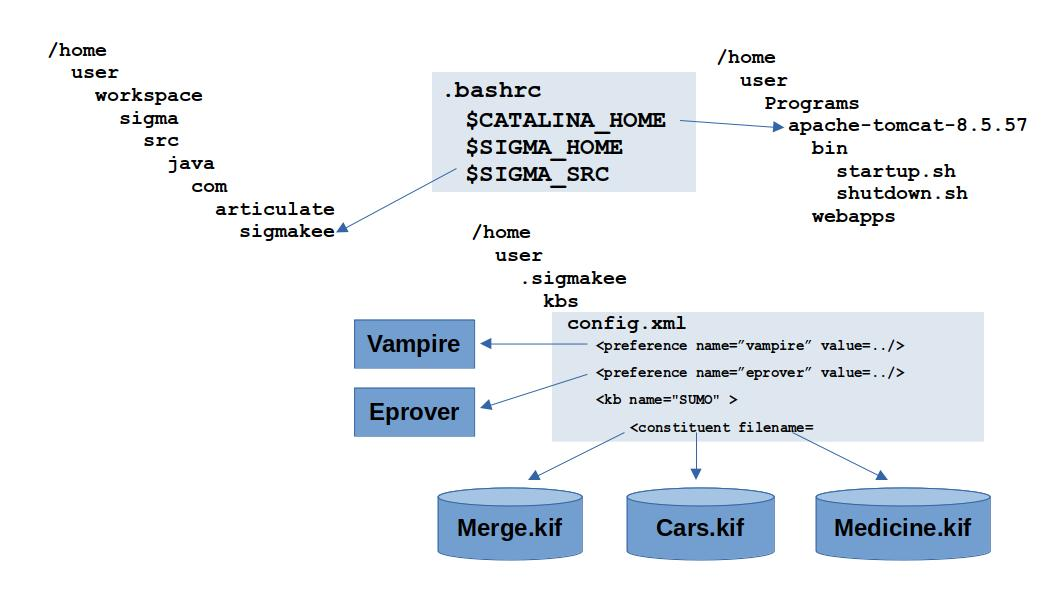
\includegraphics[width=4.5in]{pictures/config.jpg}
  \caption{Sigma configuration elements}
  \label{fig:config}
\end{figure}

Configuration of Sigma is first governed by the environment variable \texttt{SIGMA\_HOME},
which in the default configuration with point to a directory ".sigmakee" in the
user's home directory. Configuration of the Tomcat web service is governed by
the \texttt{CATALINA\_HOME} environment variable. (see Figure \ref{fig:config})

\begin{sloppypar}
The "workspace" directory will hold the Git modules for sigmakee and sumo. When
"ant" is used to compile sigma from the Git module
\texttt{/home/user/workspace/sigmakee}, it creates a \texttt{.war} file (a sort
of zip file) that is then copied to the \texttt{webapps} directory. When Tomcat
is started, it automatically expands all the \texttt{.war} files in the webapps
directory, creating the \texttt{sigma} subdirectory with all the compiled java
\texttt{.class} files and \texttt{.jsp} files.  Sigma relies on the
\texttt{SIGMA\_HOME} environment variable to find the \texttt{.sigmakee}
directory. During installation of Sigma, the user will copy SUMO \texttt{.kif}
files and SUMO-WordNet mapping files under \texttt{.sigmakee/KBs} where the
\texttt{config.xml} file also resides.
\end{sloppypar}

The \texttt{config.xml} specifies how to set many other configuration parameters
for Sigma, and which \texttt{.kif} files to load.  Sigma can have multiple named
knowledge bases loaded at one time, each of which is composed of one or more
constituent \texttt{.kif} files.  However, it's most typical just to have one
knowledge base named "SUMO".  The configuration file parameter "sumokbname" provides
the name of the file that Sigma will look for and the primary knowledege base that
is assumed at least to contain the \texttt{Merge.kif} file, which is the uppermost
level of SUMO.

\begin{sloppypar}
Default values for configuration parameters are set in
\texttt{KBmanager.setDefaultAttributes()}.
\end{sloppypar}

The full list of configuration parameters, a typical default value and their
purpose is now described:

\begin{itemize}

\item \textbf{adminBrowserLimit} - value = 200 - Each term that is viewed in the
Sigma browser can have very few or very many logical statements in which it
appears.  The term \texttt{subclass} for example, appears in tens of thousands
of statements.  To prevent the display of common terms from overwhelming the
system (and the user), Sigma limits how many are presented at each time.
Administrative users have a larger limit than guest users.

\item \textbf{baseDir} - value = \texttt{/home/user/.sigmakee} - the base data
directory for Sigma, under which the KBs directory is found.  Currently, there
are no other subdirectories.

\item \textbf{cache} - value = yes - Whether to cache transitive relationships,
using the \texttt{KBcache}\index[classes]{KBcache} class.

\item \textbf{celtdir} - Obsolete

\item \textbf{dbUser} - value = sa - The user name for the H2 database that is
currently used to store login and contact information for users of an
installation of Sigma.  Passwords are stored with 128-bit one-way encryption
only.

\item \textbf{editorCommand}  - Obsolete

\item \begin{sloppypar}\textbf{englishPCFG} - value =
\texttt{/home/user/Programs/ stanford-corenlp-full-2015-12-09} - the directory in
which the englishPCFG parser model file for Stanford's CoreNLP system is found.
This is used by the class \texttt{WSD}\index[classes]{WSD} in word sense
disambiguation\end{sloppypar}

\item \begin{sloppypar}\textbf{graphDir} - value =
\texttt{/var/tomcat/apache-tomcat-9.0.96/ webapps/sigma/graph} - the subdirectory
under which graph images will be placed\end{sloppypar}

  \item \textbf{graphVizDir} - value = \texttt{/usr/bin} - The directory in which the
executable for the open source GraphViz graph drawing software resides
\url{https://www.graphviz.org}

\item \textbf{graphWidth} - value = 600 - When a graph rendered by GraphViz is
displayed in the browser, how many pixels wide should it be?

\item \textbf{holdsPrefix} - value = no - whether to convert predicate variables
to strict first order by prefixing with \texttt{holds}

\item \textbf{hostname} - value = localhost - The value of the domain name for
the host on which Sigma is run, so it can be used in hyperlinks

\item \textbf{https} - value = false - Whether to make hyperlinks specify the
https protocol.  When true this requires that the user has configured the server
on which Sigma is running for https, including having a certificate from a
certificate authority

\item \begin{sloppypar}\textbf{inferenceEngine} - value =
\texttt{/home/user/Programs/ E/PROVER/e\_ltb\_runner} - the location of the theorem
prover executable\end{sloppypar}

\item \textbf{inferenceTestDir} - value =
\texttt{/home/user/.sigmakee/KBs/tests} - the location for a suite of inference
tests, which are files with a \texttt{.tq} extension.

\item \textbf{kbDir} - value = \texttt{/home/user/.sigmakee/KBs} - The location
where \texttt{.kif} files are read from

\item \textbf{leoExecutable}  - value = \texttt{/home/user/leo} - The location
where the LEO-II higher order theorem prover executable is found.  Note that
since this is experimental, it's not in the Sigma distribution.

\item \textbf{lineNumberCommand} - Obsolete

\item \textbf{loadCELT} - value = no - Basically obsolete now that all effort
on NLP has shifted to SigmaNLP and the Semantic Rewriting approach

\item \textbf{loadFresh} - value = false - Whether knowledge bases should be
loaded and processed from source each time Sigma and Tomcat are restarted, or if
they should be loaded from serialized files if the sources haven't been changed.
This should be kept as false unless a developer is working on changing caching
and indexing approaches.

\item \textbf{logDir}  - value = \texttt{/home/user/.sigmakee/logs} - Currently
unused, this parameter specifies where to put error and warning log files.  At
the moment, error and warnings are found in the \texttt{logs/catalina.out} file
under Tomcat.

\item \textbf{logLevel}  - value = warning - Currently unused.

\item \textbf{nlpTools}  - value = yes - Whether SigmaNLP is installed, and therefore
should have a hyperlink to it.

\item \textbf{overwrite}  - value = no - This says whether knowledge base files, when
loaded through the Manifest.jsp page, should overwrite files of the same name in the
\texttt{\$SIGMA\_HOME/KBs} directory

  \item \textbf{port} - value = 8080 - Specifies which port Tomcat should run under
for Sigma requests.  If you're running https, you'll likely use 8443 instead.  This
number gets put in the hyperlinks in the browser.

  \item \textbf{prolog} - Obsolete

  \item \begin{sloppypar}\textbf{semRewrite} - value = \texttt{/home/user/workspace/sumo/ WordNetMappings/SemRewrite.txt}
This isn't used by SigmaKEE but is used by SigmaNLP.  It probably should be in a
separate configuration file.\end{sloppypar}

  \item \textbf{showcached} - value = no - Whether to show cached statement in the browser, or
just show statements that are loaded from \texttt{.kif} files

  \item \textbf{sumokbname} - value = SUMO - The name of the SUMO knowledge base.

  \item \textbf{systemsDir} - value = \texttt{/home/user}  - Where all the TPTP theorem provers
are installed in a local installation of TPTP.  This is not exactly obsolete, but hasn't
been tested in many years, and most users will not be concerned with it.

  \item \begin{sloppypar}\textbf{testOutputDir} - value = \texttt{/var/tomcat/apache-tomcat-9.0.96/ webapps/sigma/tests}
- Where to place the results of running inference test questions.\end{sloppypar}

  \item \textbf{TPTPDisplay} - value = no - Whether to display axioms in TPTP format.  This is a bit
obsolete as it's now possible to do this from the "Formal Language" menu in the Sigma term browser.

  \item \textbf{tptpHomeDir} - value = \texttt{/home/user}

  \item \textbf{TPTP} - value = yes - This is where the TPTP framework itself, rather than the
theorem provers it communicates with, are found. Most users will not be concerned with this.

  \item \textbf{typePrefix} - value = yes - Whether to add sortal preconditions to axioms as described on
page \pageref{chap:KnowRep:subsec:Sortal}

  \item \textbf{userBrowserLimit} - value = 25 - Similar to baseDir above, but a lower
limit set for guest users

\end{itemize}

%%%%%%%%%%%%%%%%%%%%%%%%%%%%%%%%%%%%%%%%%%%%%%%%

\section{Conversion of SUO-KIF to First-Order Logic}
\label{chap:KnowRepr:sec:Conv}

Integration of the standard \index{TPTPWorld}TPTPWorld suite of theorem provers
with Sigma \cite{tsp08} and the E theorem prover \cite{Schulz:AICOM-2002}
required processing SUMO into a more strictly first-order syntax. We now discuss
the transformations that have been needed.

\small
Although not a required part of the syntax of SUO-KIF, in SUMO, by convention,
relations are written with an initial lowercase character, and functions,
non-relational instances and classes are written with initial capital letters.
\normalsize

\subsection{Predicate Variables}
\label{chap:KnowRep:subsec:PredVar}

\begin{figure}
\begin{framed}
\begin{verbatim}
(instance part TransitiveRelation)
(<=>
  (instance ?REL TransitiveRelation)
  (forall (?INST1 ?INST2 ?INST3)
    (=>
      (and
        (?REL ?INST1 ?INST2)
        (?REL ?INST2 ?INST3))
      (?REL ?INST1 ?INST3))))
\end{verbatim}
\caption{Example axioms showing predicate variables}
\label{fig:PredVarEx}
\end{framed}
\end{figure}

\begin{figure}
\begin{framed}
\begin{verbatim}
(holds instance part TransitiveRelation)
(<=>
  (holds instance ?REL TransitiveRelation)
  (forall (?INST1 ?INST2 ?INST3)
    (=>
      (and
        (holds ?REL ?INST1 ?INST2)
        (holds ?REL ?INST2 ?INST3))
      (holds ?REL ?INST1 ?INST3))))
\end{verbatim}
\caption{Example axioms with holds prefixing}
\label{fig:HoldsPrefix}
\end{framed}
\end{figure}

\begin{sloppypar}
First-order provers do not typically support variables in the predicate
position. Our first approach was to add a "dummy" predicate to all clauses other
than those with logical operators.   For example, the axioms in Figure
\ref{fig:PredVarEx}, which have the variable {\tt ?REL} in the predicate
position, become the axioms in Figure \ref{fig:HoldsPrefix}.  This transformation
is performed in \texttt{FormulaPreprocessor.preProcessRecurse()}\index[classes]{FormulaPreprocessor}.
\end{sloppypar}

This transformation however resulted in poor performance for theorem provers
that give special indexing priority to the predicate when searching the proof
space.

\begin{figure}
\begin{framed}
\begin{verbatim}
(=>
  (holds inverse ?REL1 ?REL2)
  (forall (?INST1 ?INST2)
    (<=>
      (holds ?REL1 ?INST1 ?INST2)
      (holds ?REL2 ?INST2 ?INST1))))
\end{verbatim}
\caption{"holds" insertion}
\label{fig:HoldsInsert}
\end{framed}
\end{figure}

An additional issue is that while KIF-Vampire was customized to support
variable-arity predicates, and reuse of names for both predicates and functions,
many theorem provers, such as those in the TPTPWorld suite, do not support that
flexibility.  Translation required creating new predicates for every
\index{arity}arity, and a separate set for functions, which are called {\tt
holds\_X\_\_} and {\tt apply\_X\_\_}, respectively, where X is the arity.  This
transformation has an added benefit of improving performance for those provers
which index clauses primarily on the predicate name.  The above axiom then
becomes as shown in Figure \ref{fig:HoldsArity}.

\begin{figure}
\begin{framed}
\begin{verbatim}
(=>
  (holds_3__ inverse ?REL1 ?REL2)
  (forall (?INST1 ?INST2)
    (<=>
      (holds_3__ ?REL1 ?INST1 ?INST2)
      (holds_3__ ?REL2 ?INST2 ?INST1))))
\end{verbatim}
\caption{Holds prefix with arity}
\label{fig:HoldsArity}
\end{framed}
\end{figure}

Another approach is to instantiate every predicate variable with all possible
values for predicates in the knowledge base that meet the type restrictions that
may be implied by the axiom.  The rule in Figure \ref{fig:PredVarEx} above will
be duplicated with the variable {\tt ?REL} being instantiated with every {\tt
TransitiveRelation}\index{TransitiveRelation} as in Figure \ref{fig:ExAxPred}

\begin{figure}
\begin{framed}
\begin{verbatim}
(=>
  (and
    (part ?INST1 ?INST2)
    (part ?INST2 ?INST3))
  (part ?INST1 ?INST3))
\end{verbatim}
\caption{Example axiom with predicate instantiation}
\label{fig:ExAxPred}
\end{framed}
\end{figure}

If there are ten such relations, there will be 10 copies of the axiom, each with
different values for {\tt ?REL}. This results in an automated expansion of the
number of axioms, but does give good performance.  One limitation however is
that the semantics of \index{predicate variable}predicate variables is thereby
limited to the set of predicates existing in the knowledge base, rather than
ranging over all possible predicates.

\begin{sloppypar}
This transformation is called in \texttt{FormulaPreprocessor. replacePredVarsAndRowVars()}
\index[classes]{FormulaPreprocessor}
and \texttt{PredVarInst.instantiatePredVars()}\index[classes]{PredVarInst}
does most of the actual work of the
transformation.
\end{sloppypar}

\subsection{Row Variables}
\label{chap:KnowRep:subsec:RowVar}

\begin{sloppypar}
\index{row variables}Row variables allow us to reference predicates where the
number of arguments is not known. While the unbounded implementation of the
existence of row variables would make SUO-KIF technically an "infinitary logic"
\cite{hayes2001}, with associated issues in efficient implementation, a bounded
interpretation, as described now, does keep SUO-KIF out of this problem.
\end{sloppypar}

\begin{figure}
\begin{framed}
\begin{verbatim}
(=>
  (and
    (subrelation ?REL1 ?REL2)
    (?REL1 @ROW))
  (?REL2 @ROW))
\end{verbatim}
\caption{Axiom with row variables}
\label{fig:RowVar}
\end{framed}
\end{figure}

\begin{figure}
\begin{framed}
\begin{verbatim}
(=>
  (and
    (subrelation ?REL1 ?REL2)
    (?REL1 ?ARG1))
  (?REL2 ?ARG1))

(=>
  (and
    (subrelation ?REL1 ?REL2)
    (?REL1 ?ARG1 ?ARG2))
  (?REL2 ?ARG1 ?ARG2))
\end{verbatim}
\caption{Row variable expansion}
\label{fig:RowExpand}
\end{framed}
\end{figure}

Sigma treats row variables as "macros", which get expanded
automatically so the one axiom in Figure \ref{fig:RowVar} becomes several
axioms, as shown in Figure \ref{fig:RowExpand}.  For brevity only expansion to
two variables is shown, but the expansion algorithm continues up to the maximum
arity currently allowed of 7, when appropriate.  Note that in axioms such as
this, which also require predicate variable instantiation, we must restrain the
expansion to only those arities which are compatible with the instantiated
predicates.  For example, \index{located} \texttt{located} is a
\index{subrelation} \texttt{subrelation} of \index{partlyLocated} {\tt
partlyLocated} and both have arity 2.  So, {\tt @ROW} will only be expanded to
the case of two variables. In the few cases where axioms have two row variables,
this can result in 49 new axioms.  This work happens in
\texttt{RowVars.expandRowVars()}\index[classes]{RowVars}.

\subsection{Quoting}
\label{chap:KnowRep:subsec:Quote}

The original version of KIF had an explicit single quote for denoting
uninterpreted structures that were essentially terms.  This was used to state
complex expressions which could be read by humans, without incurring the
computational cost of becoming \index{higher-order logic}higher-order logic.  For
example {\tt (believes Mary (likes John Sue))} is a higher-order expression,
because the second argument to ‘believes’ is not a term. {\tt (believes Mary
‘(likes John Sue))} is first-order in the original KIF because the single
quote character converts the following list into a term.  This however is not
strictly necessary since a reasoning system can apply a quote automatically when
needed by looking at the form of the arguments, or the domain statements which
define the argument types of the predicate.  SUO-KIF allows the unquoted
expression and leaves it to a reasoning system how it wishes to handle it.  If a
higher-order interpretation is possible, then that is allowed.  If not, then the
reasoning system is responsible for quoting any argument to a relation which is
not a term.  Sigma employs the latter approach when sending statements to its
suite of first-order logic reasoners.

Quoting removes most of the semantics of higher-order statements, including the
semantics of logical operators, but does at least allow for unification, thereby
giving the appearance of higher-order reasoning in very limited situations.

For example,

\vspace{4pt}

{\tt (believes John (likes Mary Jeff))}

\vspace{4pt}

becomes

\vspace{4pt}

{\tt (believe John `(likes Mary Jeff))}

\vspace{4pt}

This allows KIF-Vampire to perform very simple queries on higher-order
statements, such as

\vspace{4pt}

{\tt (believes John `(likes Mary ?X))}

\vspace{4pt}

and get the correct answer of Jeff.  However, logical symbols in the embedded
formulas lose their meaning, so if

\vspace{4pt}

{\tt (believes John
  '(and
     (likes Mary Jeff)
     (likes Bill Sue)))}

\vspace{4pt}

is asserted, the same query will fail, as the and does not have its conventional
meaning, and the two lists will not unify.

A better way to address these constructs is to treat them with their full higher-order
semantics.  For this we translate SUO-KIF to the THF language in the class \texttt{THF}\index[classes]{THF}
and send them to the LEO-II prover for inference.

\subsection{Sortals}
\label{chap:KnowRep:subsec:Sortal}

Provers such as KIF-Vampire are unsorted.  That is, variables may range over any
type.  However, SUMO specifies the types of arguments required for each
predicate.  When run in an unsorted prover, these specifications have the
unintended effect of generating contradictions.  Because variables can be of any
type, they may, during search, be bound to a type that is incompatible with the
restrictions on a particular predicate's argument types that are also part of
the search.  The axiom that specifies the argument type restriction for that
predicate may then contradict that \index{variable binding}variable binding.  In
addition, by allowing variables to be any type, search may include finding
bindings for variables that cannot be part of the eventual successful solution,
so there is an \index{efficiency}efficiency cost, as well as a problem for
finding an accurate \index{proof}proof.

\begin{figure}
\begin{framed}
\begin{verbatim}
(=>
  (and
    (instance ?TRANSFER Transfer)
    (agent ?TRANSFER ?AGENT)
    (patient ?TRANSFER ?PATIENT))
  (not
    (equal ?AGENT ?PATIENT)))
\end{verbatim}
\caption{Example axiom}
\label{fig:ExAx}
\end{framed}
\end{figure}

We should note that there is an efficiency cost with using sortal prefixes also,
since they increase the number of literals that must be proved in order to
derive each conclusion.  We would expect the use of sortal prefixes to improve
correctness, but at the cost of speed (and some space).  Perhaps the use of
sortals has not provided any obvious benefit so far only because we have not
allowed each test to run for a long enough time.

\begin{figure}
\begin{framed}
\begin{verbatim}
(=>
  (and
    (instance ?AGENT Agent)
    (instance ?PATIENT Object))
  (=>
    (and
      (instance ?TRANSFER Transfer)
      (agent ?TRANSFER ?AGENT)
      (patient ?TRANSFER ?PATIENT))
    (not
      (equal ?AGENT ?PATIENT)))
\end{verbatim}
\caption{Sortal prefixing}
\label{fig:SortPref}
\end{framed}
\end{figure}

To solve this problem of having search unconstrained by argument types, we
generate additional preconditions for each rule in the ontology, which then
limits every rule to being considered only if type requirements have been met.
For example, Figure \ref{fig:ExAx} is transformed into Figure
\ref{fig:SortPref}.

Note that a naïve implementation of this approach would be to state the version
in Figure \ref{fig:NaiveSort} but since {\tt ?TRANSFER} is already further
constrained by the first clause of the original rule, those additional clauses
are not necessary.

\begin{figure}
\begin{framed}
\begin{verbatim}
(=>
  (and
    (instance ?AGENT Agent)
    (instance ?TRANSFER Instance)
    (instance ?TRANSFER Process)
    (instance ?PATIENT Object))
  (=>
    (and
      (instance ?TRANSFER Transfer)
      (agent ?TRANSFER ?AGENT)
      (patient ?TRANSFER ?PATIENT))
    (not
      (equal ?AGENT ?PATIENT)))
\end{verbatim}
\caption{Naive sortal prefixing}
\label{fig:NaiveSort}
\end{framed}
\end{figure}

\begin{sloppypar}
This processing is handled in
\texttt{FormulaPreprocessor. addTypeRestrictions()}\index[classes]{FormulaPreprocessor}.
\end{sloppypar}

After these pre-processing steps are performed to transform row variables, instantiate
predicate variables and add sortal prefixes, Sigma then can translate the formulas
to the TPTP language for use in first-order theorem proving.  This is handled in
\texttt{SUMOKBtoTPTPKB}\index[classes]{SUMOKBtoTPTPKB} which then calls on \texttt{SUMOformulaToTPTPformula}\index[classes]{SUMOformulaToTPTPformula}.  The
results of this processing are stored in \texttt{Formula.theTptpFormulas}\index[classes]{Formula}.


\section{Normalization Algorithm}
\label{chap:SUMOInfe:sec:Norm}

Normalization is a process of reducing the complexity of logical formulas by
removing logical symbols which are not strictly needed.  This makes the logic
harder to read, so it's useful to be able to author knowledge in one form but
then reduce it to a simpler form for automated processing.  All modern theorem
provers work with a so-called normal form, which removes quantification and
implication symbols.  We use Russell and Norvig's algorithm \cite{RN:AI-2009}.

Normalization is handled in the class
\texttt{Clausifer}\index[classes]{Clausifier}. Sigma makes limited use of the
class, primarily just for a rare, expensive but more precise test for equality
between formulas than just looking at textual matches.  In the descriptions
below we'll provide TPTP syntax on the left and SUO-KIF syntax on the right.
Each step corresponds to a method in the code.  The top level call to
\texttt{clausify()} is

\begin{lstlisting}[basicstyle=\ttfamily\small\bfseries]
public Formula clausify() {

    thisFormula = equivalencesOut();
    thisFormula = implicationsOut();
    thisFormula = negationsIn();
    thisFormula = renameVariables();
    thisFormula = existentialsOut();
    thisFormula = universalsOut();
    thisFormula = disjunctionsIn();
    thisFormula = standardizeApart();
    return thisFormula;
}
\end{lstlisting}

\subsection{Remove implications and equivalences}

\begin{verbatim}
a<=>b is the same as        (<=> A B) is the same as
(a=>b)\&(b=>a)              (and (=> A B) (=> B A))

a=>b is the same as -a|b    (=> A B) same as (or (not A) B)
\end{verbatim}

\subsection{Move negation inwards}

\begin{verbatim}
-(p|q) becomes -p\&-q           (not (or P Q)) becomes
                                (and (not P) (not Q))

-(p\&q) becomes -p|-q           (not (and P Q)) becomes
                                (or (not P) (not Q))

-![X]:p becomes ?[X]:-p	        (not (forall (?X) P)) becomes
                                (exists (?X) (not P))

-?[X]:p becomes ![X]:-p	        (not (exists (?X) P)) becomes
                                (forall (?X) (not P))

--p becomes p                   (not (not P)) becomes P
\end{verbatim}

\subsection{Standardize variables}

The scope of variables in quantifiers is local to the quantifier, but to avoid
confusion, variables of the same name but different scope in a formula are
renamed.

\begin{verbatim}
![X]:p(X)|?[X]:q(X) becomes          (or
![X]:p(X)|?[Y]:q(Y)                    (forall (?X)
                                         (p ?X))
                                       (exists (?X)
                                         (q ?X)))
                                     becomes

                                     (or
                                       (forall (?X)
                                         (p ?X))
                                       (exists (?Y)
                                         (q ?Y)))
\end{verbatim}

\subsection{Move quantifiers left}

\begin{verbatim}
p|![X]q(X) becomes         (or P (forall (?X) (q ?X))) becomes

![X]p|q(X)                 (forall (?X) (or P (q ?X)))
\end{verbatim}

\subsection{Skolemization}

Create a unique function in place of every existentially quantified variable.
Include every universally quantified variable that is in scope, inside the
function.

\begin{verbatim}
![X]:p(X) =>                     (forall (?X)
    (?[Y]:h(Y) \& a(X,Y))          (=>
                                     (p ?X)
                                     (exists (?Y)
                                       (and
                                         (h ?Y)
                                         (a ?X ?Y)))))
\end{verbatim}

becomes

\begin{verbatim}
![X]:p(X) => 	            (forall (?X)
    (h(skf(X)) \&           (=>
     a(X,skf(X)))             (p ?X)
                              (and
                                (h (skf ?X))
                                (a ?X (skf ?X))))
\end{verbatim}


\subsection{Distribute and over or}

\begin{verbatim}
(a \& b) | c becomes     (or (and a b) c) becomes
(a | c) \& (b | c)       (and (or a c) (or b c))
\end{verbatim}

\subsection{Flatten nested conjunctions and disjunctions}

\begin{verbatim}
(a | b) | c becomes     (or (or a b) c) becomes
a | b | c               (or a b c)
\end{verbatim}



\section{Conversion to TPTP}
\label{chap:SUMOInfe:sec:Conv}

While the conversions described above result in an essentially first-order form,
there are several aspects that are beyond the "traditional human-readable"
format of the TPTP language, as parsed by many current provers. The TPTP
language uses \index{Prolog}Prolog-like user terms and atoms, uses infix
notation for binary operators, has a separate namespace for operators, and
provides a separate namespace for defined functors and predicates. Additionally
the TPTP language does not support arbitrary lists. These differences are dealt
with in the translation to TPTP format as follows.

A recursive algorithm is used to convert from the SUO-KIF prefix form for binary
operators, stacking the translated form of an operator when found at the start
of a formula, copying it off the top of the stack for insertion between operand
formulae, and popping it off the stack at the end of the formula. As user terms
and atoms are encountered they are translated to Prolog’s prefix form, with
functors’ and predicates’ first letters being set to lowercase, and
variables’ first letters being set to upper case. All hyphens in user terms
are translated to underscores. Functions, recognized in SUO-KIF by the "Fn"
suffix, are translated to corresponding equivalents from the TPTP language,
starting with a "\$". A minor translation of double quoted strings is
performed, replacing non-printable characters - carriage return, new line, tab,
and formfeed - by spaces.

Truly higher-order
constructs are dealt with by losing most of their semantics by conversion to
uninterpreted lists. This translated form is not directly usable in the TPTP
format, as there is no support for arbitrary lists. The current solution is to
lose even more of the semantics, by single quoting such expressions, thus
treating them as constants. In this way the possibility of unification over the
list elements is lost - only unification of the whole is possible. Part of the
reason for taking this simplistic approach was to permit consistent translation
of operators, and because they have a separate namespace in the TPTP language
they cannot be treated as terms in a list. The list solution can be implemented
in the translation to TPTP format by retaining the SUO-KIF forms of operators
(which look like TPTP constants), adding the {\tt \_X\_\_} suffix to the
predicate list to form unique predicates for different arities at the atom
level, and providing {\tt listf\_X\_\_} functors for nested lists.

%%%%%%%%%%%%%%%%%%%%%%%%%%%%%%%%%%%%%%%%%%%%%%%%

\chapter{Using Sigma}
\label{chap:UsingSigma}



\section{JSP Interface}
\label{chap:KnowEngi:sec:JSPInterface}

Sigma has a number of functions controlled through its JSP-based interface.  Sigma
runs under Tomcat, which is a web server that allows Java code to be embedded in
HTML pages and run on the server, as opposed to JavaScript, which is run on the
client.

\begin{itemize}

\item AddConstituent.jsp - adds a constituent SUO-KIF file to a knowledge base.  Accessible only to
admin users.  It just responds to a command from another page and has no UI of its own.
Redirects back to KBs.jsp when done.

\item AllPictures.jsp - shows all the pictures linked to a term at once.  Accessible to all users.

\item ApproveUser.jsp - handles approving a new user.  Accessible only to admin users. Redirects
to KB.jsp once acknowledge.

\item AskTell.jsp - interface to the local theorem provers. Accessible only to admin users. This function
has not been well maintained and the interfaces to SystemOnTPTP and LEO-II may be out of date.

\item BrowseBody.jsp - shows terms, axioms, lexicon links, etc

\item BrowseExtra.jsp - includes Prelude.jsp and Postlude.jsp

\item BrowseHeader.jsp - primary ontology browser controls including term and word search, as well as
the menu for selecting natural language and formal language

\item Browse.jsp - top level browsing JSP that includes Prelude.jsp, BrowseHeader.jsp, BrowseBody.jsp
and Postlude.jsp.  Really just a shell for the included JSPs

\item CCheck.jsp - interface to \texttt{KBmanager.initiateCCheck()} that initiates consistency checking of a KB.
Handles selection of which theorem prover to use, and several parameters.  Includes Prelude.jsp
and Postlude.jsp

\item CELT.jsp - Obsolete.  Handles invocation of the Controlled English to Logic Translation system,
which is now superceded by the Semantic Rewriting approach in the sigmanlp project.

\item CreateUser.jsp - handles a request from a user to create an account.  Creates a guest account
and sends mail to the moderator for approval.  Has no UI.

\item Diag.jsp - Interface to run tests in Diagnostics.java.  Depends on Prelude.jsp and Postlude.jsp.
Accessible for "admin" and "user" but not unregistered guest users

\item EditFile.jsp - Obsolete

\item EditStmt.jsp - Obsolete

\item Graph.jsp - Create graphs of binary relationships as a graphical view and as indented text.
Relies on Prelude.jsp and Postlude.jsp

\item InferenceTestSuite.jsp - run a suite of inference tests with the prover and parameters selected.
Depends on Prelude.jsp and Postlude.jsp.  Accessible only for admin users.

\item init.jsp - A status page with periodic automatic refresh to catch requests to Sigma during the
process of initialization.

\item InstFiller.jsp - Page to allow simple editing of ground formulas.  Deprecated.  Accessible only
for admin users. Depends on Prelude.jsp and Postlude.jsp.

\item Intersect.jsp - Find appearances of two or more terms in the same axiom.  Depends on
Prelude.jsp and Postlude.jsp.

\item KBs.jsp - Main entry point for creating or selecting a knowledge base.  Some functions are
available for "admin" or "user" roles but not "guest". Depends on Prelude.jsp and Postlude.jsp.

\item login.html - login page for Sigma that handles existing accounts and new account registration.
Existing accounts are dispatched to login.jsp and registrations are dispatched to
Registration.jsp

\item login.jsp - handle the login process by using PasswordService.jsp to validate a login against
an H2 database of account info.  This page has no UI.

\item Manifest.jsp - UI for handling loading and saving KB constituents including saving in various
exportable formats, such as OWL. Depends on Prelude.jsp and Postlude.jsp. Most functionality
is limited to admin users.

\item Mapping.jsp - Use some simple string matching approaches to suggest equivalences between terms
in two files.  Depends on Prelude.jsp and Postlude.jsp. Access limited to admin users.

\item MiscUtilities.jsp - Depends on Prelude.jsp and Postlude.jsp. Most functionality
is limited to admin users. Little utilities to generate dot graph files and OWL versions of
the Open Multilingual Wordnet content.

\item ModeratorApproval.jsp - Functionality is limited to admin users. Dispatches to ApproveUser.jsp
when user clicks "ok".

\item OMW.jsp - Display results from the many languages in Open Multilingual Wordnet linked to
WordNet synsets. Depends on Prelude.jsp and Postlude.jsp.

\item OWL.jsp - Display all the axioms for a given term in OWL format, if expressible in that
language.

\item Postlude.jsp - Encapsulates footing information displayed on most pages.

\item Prelude.jsp - Encapsulates header information displayed on most pages.

\item ProcessFile.jsp - No UI. Called from MiscUtilities.jsp to generate KIF from other
formats. Calls \texttt{DocGen.dataFileToKifFile()} to do the real work. Depends on Prelude.jsp and
Postlude.jsp. Access limited to admin users.

\item Properties.jsp - An interface for setting many of Sigma's parameters.  Some of these are
also accessible from the browsing interface, such as the language for the natural
language paraphrases. Depends on Prelude.jsp and Postlude.jsp. Access limited to admin users.

\item Register.jsp - An interface to allow people to submit a request for registration and
priviledges beyond that of unregistered guest users.  Calls on CreateUser.jsp

\item Save.jsp - not used

\item SimpleBrowseBody.jsp - Analogue to BrowseBody.jsp but showing only simple axioms in a simple
and non-technical language

\item SimpleBrowseHeader.jsp - Analogue to BrowseHeader.jsp for simple axioms

\item SimpleBrowse.jsp - Analogue to Browse.jsp for simple axioms

\item SystemOnTPTP.jsp - Interface to the SystemOnTPTP system hosted as U. Miami that collects
dozens of theorem provers with a common programmatic interface.  This code has not been
maintained so use at your own risk. Depends on Prelude.jsp and Postlude.jsp. Access
limited to admin users.

\item TreeView.jsp - A simple tree view of the taxonomic structure of the ontology with collapsable
nodes.  Uses the SimpleBrowse.jsp code to display axioms for any node in the taxonomy.

\item WNDiag.jsp - Diagnostics for WordNet. Depends on Prelude.jsp and Postlude.jsp. Accessible
for "admin" and "user" but not unregistered guest users.

\item WordNet.jsp - show synsets and SUMO-WordNet mappings for a word. Depends on Prelude.jsp
and Postlude.jsp.

\item WordSenseFile.jsp - show word sense disambiguation and sentiment analysis results for a
file of text.  Calls \texttt{WordNet.wn.sumoFileDisplay()} for the real work. Depends on
Prelude.jsp and Postlude.jsp.

\item WordSense.jsp - show word sense disambiguation and sentiment analysis results for a
sentence.  Calls \texttt{WordNet.wn.sumoSentenceDisplay()} for the real work. Depends on
Prelude.jsp and Postlude.jsp.

\end{itemize}

\section{Language Generation}
\label{chap:KnowEngi:sec:LangGene}

SUMO proper has a significant set of manually created language display templates
that allow terms and definitions to be paraphrased in various natural languages,
including those with non-western character sets.  This approach was first
developed in \cite{DBLP:conf/kes/Sevcenko03}. These templates now include
Arabic, French, English, Czech, Tagalog, German, Italian, Hindi, Romanian and
Chinese (traditional and simplified characters). Automatically generated natural
language paraphrases can be seen in the rightmost column of the screen display
given as Figure \ref{fig:SigmaScreen}.

\begin{figure}
  \centering
  \includegraphics[width=4.5in]{pictures/SigmaScreen.png}
  \caption{Sigma browser screen}
  \label{fig:SigmaScreen}
\end{figure}

This functionality is implmeneted in the \texttt{com.articulate.sigma.nlg}
package, primarily in the \texttt{LanguageFormatter}\index[classes]{LanguageFormatter} class.  There is an
expanded approach for NLG in the remaining classes in the package, but it is
not fully implemented so those classes should be ignored for now.

Although presentation of terms is straightforward, presentation of statements is
more complicated, and roughly patterned after C-language \index{printf}printf
statements. For example the relation part, which states that one object is a
part of another, has the corresponding language generation template "\%1 is \%n
a part of \%2". The first argument to the logical relation is substituted for
\%1 etc. Note that this substitution is recursive, so that complex statements
with nested formulae can be translated effectively. The \%n signifies that if
the statement is negated, that the negation operator for the appropriate human
language should be inserted in that position.

The predicate format associates a concept (either a relation or a function) with
a string.  format takes three arguments: the name or abbreviation of a natural
language, the relation name and the format string.  When there is a need to
render a concept in natural language, the associated string is used.  The string
contains a natural language description of the concept and special tags which
are interpreted with the browser.

Take for example that we have the SUO-KIF statement that

\begin{verbatim}
(authors Dickens OliverTwistBook)
\end{verbatim}

We have the following statements that have been coded to support the
paraphrasing of statements with the authors relation.

\begin{verbatim}
(format EnglishLanguage authors
  "\%1 is \%n the \&\%author of \%2")
(format it authors "\%1 è l' \&\%autore di \%2")
\end{verbatim}

Terms are also given language-specific strings, when appropriate

\begin{verbatim}
(termFormat EnglishLanguage OliverTwistBook "Oliver Twist")
\end{verbatim}

If a Sigma user has loaded this information in a knowledge base, and English is
selected as the presentation, the user will see "Dickens is the author of Oliver
Twist." next to the SUO-KIF statement.  If Italian is selected, the paraphrase
will be "Dickens è l'autore di Oliver Twist".  As mentioned above, the %n
refers to the word for negation in the given language, and is inserted if the
formula is negated.  For example,

\begin{verbatim}
(not (authors RobinCook WarAndPeace))
\end{verbatim}

is rendered as "Robin Cook is not the author of War and Peace." The full
description of tags that may be included in the format statements is as follows:

\begin{itemize}

\item \&\%token – specifies a token that will be made into a hypertext link to
the concept being visualized.

\item \%1, \%2, ... – this tag will be substituted with a natural language
representation of the concept’s respective argument.

\item \%n{text} – will be replaced either with an empty string, if a predicate
is being rendered as positive, or "text" otherwise; the \%n tag can be used as a
shortcut for \%n{not}. \%p{text} – will be replaced with "text" for positive
rendering and with an empty string for negative rendering.

\item \%*{range}[delim] – will be replaced with a list of natural-language
representations of a subset of arguments; range specifies which arguments will
be included; it is a comma separated list of numbers or ranges, for example,
"1-4,6" denotes the first, second, third, fourth and sixth argument; the
delim parameter specifies the delimiter which will be used to separate
representations of arguments; both {range} and [delim] may be omitted, in which
case {range} defaults to all arguments, and [delim] defaults to a single space.

\item \%\% – will be replaced with a single percent character.
\end{itemize}

This is a simple approach that works reasonably well for English, but which does
not work well for languages with more types of grammatical agreement.

More recently, we have developed an approach to improve the translation of
axioms involving variables.  Variable names can be any string, but as they are
often given the form of English words, it was confusing to present the names
unaltered in presentations other than English. The solution was to collect the
types of variables and use that type as its name.  Take for example the axiom in
Figure \ref{fig:Ambulating}.

\begin{figure}
\begin{framed}
\begin{verbatim}
(=>
    (and
        (instance ?AMBULATE Ambulating)
        (agent ?AMBULATE ?AGENT))
    (attribute ?AGENT Standing))
\end{verbatim}
\caption{An axiom for {\tt Ambulating}}
\label{fig:Ambulating}
\end{framed}
\end{figure}

Sigma will generate the following English paraphrase: "If a process is an
instance of ambulating, and an agent is an agent of the process, then standing
is an attribute of the agent."

Sigma checks the argument type restrictions of the relations to determine the
type of the variables.  For example, the first argument of the agent relation is
an instance of a {\tt Process} and the second argument is an instance of an {\tt
Agent}. Sigma uses the termFormat expression for {\tt Process} to generate the
string process".  If instead the user had asked for an Italian paraphrase the
string processo" would be the result.  This is preferable to the old version of
the natural language paraphrase in which the user would have seen the variable
name {\tt ?AMBULATE} even if a non-English paraphrase was requested.

\section{Browsing and Display}
\label{chap:KnowEngi:sec:Brow}

Sigma was originally just a display tool. Its original, and still most heavily
used function, is for creating hyperlinked sets of formatted axioms that all
contain a particular term (Figure \ref{fig:SigmaScreen}). Clicking on a term in
turn gives a hyperlinked display of all the axioms that contain the new term.
Next to each axiom is given the file and line(s) where the axiom was written.
Also shown is an automatically generated natural language paraphrase of each
axiom.

\begin{figure}
  \centering
  \includegraphics[width=4.5in]{pictures/SigmaSimp.png}
  \caption{Simplified browser view}
  \label{fig:SigmaSimp}
\end{figure}

A simplified browser view (Figure \ref{fig:SigmaSimp}) that may
be more appropriate for users who are transitioning from use of frame and
\index{description logic}description logic languages.  It gives prominence to a
tree view of the subclass hierarchy and presents binary relations in a simple
tabular format, relegating rules to an area lower in the browser pane, and
rendering them in the natural language paraphrase form only.

SUMO has several hierarchies that can be used to organize and display the
theory.  These include hierarchies of physical parts, relations, attributes,
processes and others.  As such, the tree browser allows the user to select any
\index{transitive binary relation}transitive binary relation as the link by
which the hierarchy display is created.

Images provide an informal visual representation of as many of the concepts in
SUMO as possible.  Some 12,000 links were made by hand to public domain icons
and images in \index{Wikipedia}Wikipedia.  Some 900 images linked to Wikipedia in
Princeton's \index{ImageNet}ImageNet \cite{deng2009} corpus were also imported.

\section{Analysis and Debugging}
\label{chap:KnowEngi:sec:Anal}

Sigma includes a number of specialized and general tools for ensuring ontology
quality. These are contained in the
\texttt{Diagnostics}\index[classes]{Diagnostics} class. The ultimate tool for
quality checking on a formal ontology is formal reasoning.  However, in
expressive ontologies, such as SUMO, we can generally not expect that all
\index{contradiction}contradictions can be detected with theorem provers or that
consistency can be formally proved (note, for example, that Peano arithmetic can
be formalized in SUO-KIF). Sigma
therefore provides different tools for quality checking, combining exhaustive
and terminating special purpose tests with incomplete and generally
non-terminating general purpose testing based on theorem proving or model
finding.

There are two special case tests for errors that must be corrected.  We test for
terms without a root in the subclass hierarchy at the term {\tt Entity}, which
is the topmost term in SUMO (in \texttt{Diagnostics.termsNotBelowEntity()}).
This commonly results from either omitting a subclass or instance statement when
defining a new term, or by misspelling the name of the intended parent term. The
second special case test is for where a term has parents that are defined to be
disjoint (in \texttt{Diagnostics.childrenOfDisjointParents()}).  In a large
theory like SUMO, it can be easy to lose track of this case, especially when the
ultimate conflict may be between terms that are many levels up in the subclass
hierarchy.

\begin{sloppypar}
There are also a number of tests for cases that are indicative of a problem, yet
not strictly an error that would result in a logical contradiction.  The first
of these is for terms lacking documentation (in
\texttt{Diagnostics.termsWithoutDoc()}).  In theories under construction,
theories that are the results of importing and merging another ontology, or
simply for large lists of domain instances, like city names, it may be
reasonable, temporary, or expected for such terms to lack documentation.  But
this does often reflect an outright error, where a term name was simply
misspelled in the documentation definition, or in some other axiom.  The test
\texttt{Diagnostics.termsWithMultipleDoc()} may also be indicative of a problem, as
can relations without any natural language \texttt{format} expression (checked in
\texttt{Diagnostics.relationsWithoutFormat()}).
\end{sloppypar}

We test for cases where terms do not appear in any rules (in
\texttt{Diagnostics. termsWithoutRules()}).  This again is common in collections
of instance-level facts, but undesirable for many classes or relations, where it
should be possible to define precisely the intended meaning of the term with a
small number of formal rules, as well as statements like class membership.

Rules can be syntactically valid with quantified variables that appear in a quantifier
list but aren't used in the scope of the quantifier.  These can be found
with \texttt{Diagnostics.quantifierNotInBody()} and are often indicative of
a typo in the variable name.

\begin{sloppypar}
A more complicated issue is where members (instances) of a parent class that are
not also members of one of the subclasses that constitute the exhaustive
decomposition of the parent class (stated with the relation
\texttt{exhaustiveDecomposition}).  This problem is found with
\texttt{Diagnostics.membersNotInAnyPartitionClass()}.
\end{sloppypar}

Because knowledge bases are often composed from SUMO's general and domain
specific component ontologies, it is desirable to limit dependencies among the
files as much as possible.  For that reason we include a tool to specify
dependencies between pairs of files (in
\texttt{Diagnostics.printTermDependency()}).  It is typically most desirable at least to
ensure that dependencies are only from one file to another, and not between both
files.  All domain files will of course depend at least upon SUMO proper, since
they form a single integrated theory that is decomposed into separate files for
convenience and efficiency of inference.

A further test exploits the SUMO-WordNet mappings. They offer the opportunity to
find problems exposed by differences in the two products.  The two hierarchies
should not necessarily be isomorphic, and therefore respective differences do
not necessarily mark an error, but are worth examination when they are found.

\begin{sloppypar}
In the \index{diagnostics}diagnostics provided for the SUMO-WordNet mappings
(found in \texttt{WNdiagnostics}\index[classes]{WNdiagnostics}), Sigma finds
WordNet synsets without mapped formal terms (in
\texttt{WNdiagnostics.synsetsWithoutTerms()}) and those for which a formal term
is provided, but is not found in the current loaded knowledge base (in
\texttt{WNdiagnostics.synsetsWithoutFoundTerms()}). This helps to find cases
where terms have been changed or renamed and the mappings not updated. There is
also a reverse case of where a SUMO term doesn't have a synset. Relations in
SUMO (including functions) won't have mappings.  There are also terms in SUMO,
especially the domain ontologies, which are too specific to have a mapping -
only their parent terms in SUMO are mapped and therefore their mapping can be
inferred.  This case is checked for in
\texttt{WNdiagnostics.nonRelationTermsWithoutSynsets()}.
\end{sloppypar}

Most significant is the taxonomy comparison component. Given that we have terms
A and B in SUMO and synsets X and Y in WordNet, if A is mapped to X and B to Y,
Sigma checks whether if B is a subclass of A then Y is also a hyponym of X. The
reverse case is also checked.  This test is found
in\texttt{WNdiagnostics.nonMatchingTaxonomy()}.

\section{Inference}
\label{chap:KnowEngi:sec:Infe}

\begin{sloppypar}
The SUMO Inference Engine (\index{SInE}SInE) \cite{DBLP:conf/cade/HoderV11},
which selects only the subset of axioms likely to be relevant for a given query.
The algorithm is implemented in the SInE class\index[classes]{SInE}.  Results
show dramatic improvement on SUMO-based inference over other approaches
\cite{ps07}. We should note however that this class is only useful if one wanted
to implement a connection to a prover other than Vampire or Eprover, as both of
them have incorporated with SInE algorithm since its performance advantage was
immediately clear on large knowledge bases.
\end{sloppypar}

We have the class \texttt{InferenceEngine}\index[classes]{InferenceEngine} to
structure interaction with theorem provers.  The class
\texttt{EProver}\index[classes]{EProver} handles interaction with E.  Most users
will not need the \texttt{Vampire}\index[classes]{Vampire} class, since it only
interfaces with KIF-Vampire which is now over a decade old.  However, the
\texttt{SystemOnTPTP}\index[classes]{SystemOnTPTP} class can be used to
interface with the latest Vampire and over 40 other provers, albeit in a
somewhat more heavyweight fashion of remote communication to the TPTP servers at
U. Miami or by replicating their server installation locally.

In addition to preprocessing, some post-processing is needed for all theorem
provers that are used in Sigma.  All the TPTP provers that report full proofs,
as well as KIF-Vampire, present an ordered list of deductions, where premises
are given and then a conclusion.  In presenting a proof to the user (Figure
\ref{fig:SigmaProof}), we would like to avoid showing the same axiom many times
if it is used in several proof steps.  We therefore assign a numerical index to
each axiom, in order of its appearance in the proof.  The indexes can then be
referenced when they are preconditions to a listed step, making the proof appear
more similar to what a logic student will be used to from a standard textbook
presentation of a proof.

\begin{figure}
  \centering
  \includegraphics[width=4.5in]{pictures/SigmaProof.jpg}
  \caption{Proof presentation in Sigma, from \cite{tsp08}}
  \label{fig:SigmaProof}
\end{figure}

An answer variable is a binding for a variable in a query that is unbound. In
the proof shown in Figure \ref{fig:SigmaProof} {\tt ?X} is an unbound variable
in the query. For TPTP systems that do not report answer variables, or handle
more than one answer per query, a more complicated approach is needed.  For
systems such as EP, that report proofs but not answer variables, the axioms in
the proof are resubmitted to the \index{Metis}Metis prover
\cite{hurd2003firstorder} which does report answer variables.  Multiple answers
are found by resubmitting the query with a new clause added that excludes
previous answers.  For the example query shown in Figure \ref{fig:SigmaProof},
in order to get the second answer, the new query would become as shown in Figure
\ref{fig:NegQuery}.

\begin{figure}
\begin{framed}
\begin{verbatim}
(and
  (instance ?X PrimaryColor)
  (not
    (equals ?X Red)))
\end{verbatim}
\caption{New query, negating the first result in order to find a new answer.}
\label{fig:NegQuery}
\end{framed}
\end{figure}

At the boundary of diagnostics and inference we have the general case of using
theorem proving to find contradictions.  Because first-order proving is not
guaranteed to find all problems that may exist in SUMO, Sigma includes a
consistency check function that leads the theorem prover to consider each axiom
in a knowledge base. This is an important point because a user may have a
knowledge base that is inconsistent, but in practice may make many useful
inferences over a long period of time while never having the problem show up in
a proof. For example, take the knowledge base shown in Figure \ref{fig:ContKB}.

\begin{figure}
\begin{framed}
\begin{verbatim}
(fatherOf John Bill)
(fatherOf John Mark)
(=>
  (fatherOf ?X ?Y)
  (and
    (not
      (exists (?Z)
        (and
          (fatherOf ?X ?Z)
          (not
             (equal ?Y ?Z)))))))
\end{verbatim}
\caption{Example contradictory knowledge base}
\label{fig:ContKB}
\end{framed}
\end{figure}

While this knowledge base is trivially small, imagine that there are tens or
hundreds of thousands of other statements, many of which may involve the
predicate symbol {\tt fatherOf}.  A complete examination of the proof space is
impossible.  Imagine that the user poses the query

\begin{verbatim}
(fatherOf John Bill)
\end{verbatim}

Given a finite and small amount of time with which to find an answer, the prover
may just find and return "yes" after encountering the first assertion.  It may
not continue the search process to find the contradiction.  In fact, given a
large and complex enough knowledge base, and a complex enough contradiction, it
might not be found for years.

To help guide the search for contradictions, Sigma takes each axiom, which is
loaded one by one starting with an empty knowledge base.  For each axiom, the
prover is asked to compute whether the knowledge base contradicts the axiom, or
is redundant with it.  If the axiom doesn't create a contradiction, it is
asserted to the knowledge base and the next axiom is considered.  A
contradiction will stop processing, since once a contradiction is found, any
further results may be nonsensical (although the answer also may not be
nonsensical, as we have explained, so this is a conservative approach).

Once processing finishes, redundancies are collected and reported.  At its
simplest, a redundancy can be a duplicated statement, and that is clearly an
error. Although initially harmless, having the same statement in two places can
easily lead to problems as an ontology evolves, as one statement might get
changed while a duplicate does not.  For example, a developer might forget that
a domain ontology file already has a statement {\tt (subclass Table Furniture)}
and assert the same statement in a different file.

A more complex case is where one statement is simply deducible from several
others.  This is often intentional, as knowledge engineers may wish to
short-circuit a common chain of reasoning in order to have faster inference.
Such a case is even more likely to suffer from the problem of changes not being
reflected in the chain of deductions, and the redundant conclusion.  For
example, see Figure \ref{fig:RedunKB}.

\begin{figure}
\begin{framed}
\begin{verbatim}
(subclass Table Furniture)
(subclass DiningTable Table)
(subclass DiningTable Furniture)
(=>
  (instance ?P TransitiveRelation)
  (=>
    (and
       (?P ?A ?B)
       (?P ?B ?C))
    (?P ?A ?C)))

(instance subclass TransitiveRelation)
\end{verbatim}
\caption{Example redundant knowledge base}
\label{fig:RedunKB}
\end{framed}
\end{figure}

Similar to the \index{CASC}CASC competition, but on a much smaller scale, Sigma
has the capability to run a series of SUMO-based tests for any theorem prover it
supports, reporting success or failure and the time taken on each test.  This is
handled in the \texttt{CCheck}\index[classes]{CCheck} and \texttt{CCheckManager}\index[classes]{CCheckManager} classes.


\section{Proof Presentation}
\label{chap:SUMOInfe:sec:Proo}

Sigma includes several options for proof presentation. Despite the fact that
most textbooks present proofs as linear structures, proofs are trees. The same
sub-proof may be used several times in reaching different intermediate
conclusions. In order to ease the understanding of Sigma proofs for humans,
Sigma's proof linearization mechanism therefore integrates tools that detect and
eliminate repetitions of identical sub-proofs.

\begin{sloppypar}
When using the TPTP system integrated into Sigma, the user also has the option
of a graphical proof presentation with the IDV component \cite{trac2007}.
\end{sloppypar}

Sigma has options for how it presents multiple proofs. Often, the same proof,
with the same proof steps, can be reached via a different search order. This
means that although two tree-structured proofs may be different, they may work
out to be identical when redundant paths are removed and a linear proof
structure generated. Sigma supports an option for hiding such duplicate proofs.
One additional option is to suppress proofs that may have different steps but
which lead to the same answer. Sometime it is useful to a knowledge engineer to
see these alternate proofs, and sometime not.

Proofs are handled in the classes
\texttt{ProofProcessor}\index[classes]{ProofProcessor} and
\texttt{ProofStep}\index[classes]{ProofStep}.


\section{Mapping, Merging and Translation}
\label{chap:KnowEngi:sec:Mapp}

In addition to SUO-KIF and TPTP syntax, Sigma can also read and write OWL format
\cite{bechhofer2004owl}. Since many lightweight ontologies are currently being
created in OWL, this feature opens up the use of Sigma to a large community, and
provides a straightforward migration path to use of a more expressive logic and
more sophisticated inference.  It also opens up the use of SUMO to a community
that wishes to have simple and fast inference, since SUMO can be (and is)
exported with a lossy translation to an OWL version.  While the bulk of the SUMO
axioms are not directly expressible in OWL, they can serve as informative
comments (and in fact are exported as human-readable comments) that serve to
better define terms for the human user than if they were simply omitted.

Sigma also includes an export of facts in \index{Prolog}Prolog form.  Once Sigma
generates a TPTP version of an ontology, the TPTPWorld tools also handle a
translation to Prolog that supports horn clause rules. There is also a simple
prototype capability for exporting SQL statements for database creation and
population from Sigma.

The growing availability and coverage of lightweight taxonomies that cover
domain specific knowledge, and the corresponding phenomenon of "\index{linked
data}linked data" as a community objective has encouraged the addition of an
ontology mapping and merging capability to Sigma.  It is based on earlier work
on a stand-alone tool \cite{li2004lom}.  In mapping SUMO to simple taxonomies
there is often very little information for the machine to use to determine what
matches might exist. The principal problem appears to be massive numbers of
false positive matches. A simple algorithm appears to do as well in practice as
a more sophisticated one, since the bulk of effort is still spent by a human in
selecting accurate matches.  Having a simple and easy user interface appears to
provide more leverage than an incrementally better matching algorithm.


\section{Working with Sigma and SUMO}
\label{chap:KnowEngi:sec:Work}

There are as many possible processes for formal ontology development as there
are for software development.  Small projects may benefit from the low overhead
of an informal process.  Large projects with big teams will benefit from a
greater degree of formal process.  A typical process employing Sigma to extend
SUMO is as follows:

\begin{itemize}

\item Developers use a set of instructions or documents as a source, or write
down text in natural language that describes the domain of interest.

\item The text is used as a basis for creating a glossary of natural language
terms and definitions Developers examine the SUMO hierarchy (using the term
browser, and tree/graph browser) for each term in the glossary. The WordNet
search pages are used to find all the different meanings of each defined word in
the source text, and the WordNet-SUMO mappings are used to find the formal SUMO
term that best fits the intended meaning of the textual term.  For any
substantially new and specialized domain, the task is to find a more general
term that encompasses the meaning of the more specific textual term. Textual
terms that are already covered by specific SUMO definitions are put aside as
complete. For new terms and definitions that are needed, developers begin by
adding subclass or instance statements to the appropriate leaf term in SUMO, by
creating and editing a text file in SUO-KIF format.

\item Once a preliminary SUO-KIF file has been created, developers load it into
Sigma, along with SUMO proper and all the other domain ontologies the new file
may extend. Developers run the Sigma \index{diagnostics}Diagnostics to find any errors.

\item Developers use the information in the natural language definitions created
earlier to guide creation of SUO-KIF axioms. Each class should have at least a
subclass statement and a documentation statement. Each relation should have
domain statements defining the class membership of its arguments, and be defined
as an appropriate type of relation, such as {\tt
TransitiveRelation}\index{TransitiveRelation}. Each term should have at least
one rule, that helps to make the term usable for inference. If there are very
few things that can be stated about the term, reconsider whether it should be
created.

\item Developers create {\tt format}\index{format} and {\tt
termFormat}\index{termFormat} statements in the language of choice to support
natural language paraphrases in Sigma for the axioms previously written. These
can be presented to domain experts to help confirm that the desired knowledge
has been captured correctly. Developers map the terms in the ontology to
WordNet. This is accomplished by placing links in the existing SUMO-WordNet
mapping files (if mapping to English) that update the existing links where
needed to point to the more specific terms that have just been created
Developers load the revised WordNet mapping files into Sigma and use the Sigma
WordNet Diagnostics to see where the WordNet hierarchy may differ from the
formal relationships created in the new ontology. The existence of differences
is not necessarily bad, but they should be examined and understood.

\item Developers run the Sigma \index{Consistency Check}Consistency Check to
find any logical contradictions in the new theory.   Normally, there will be
many cycles of adding content, then running the Diagnostics and Consistency
Check processes in Sigma to find and correct errors as the theory is elaborated.
At each iteration where no errors are found, in a group development process, the
theory would be uploaded to a source configuration management system such as
\index{CVS}CVS or \index{Subversion}Subversion. Other developers are then free
to test new theories with respect to their own work, and coordinate with each
other.  One can view the Diagnostics and Consistency Check steps as analogous to
compilation and build of a conventional procedural computer program.

\item \index{peer review}Peer review is one of the best ways to improve a
theory. Sigma helps developers significantly beyond just reviewing a file of
declarative code, allowing them to search and test a theory in many different
ways.

\end{itemize}

\section{Browsing and Editing}
\label{chap:KnowEngi:sec:BrowEdit}

The Sigma system contains several different sorts of browsers for viewing formal
knowledge bases. The most basic component is a term browser, which presents all
the statements in which a particular term appears. The statements are sorted by
argument position and then the appearance of the term in rules and non-rule
statements are then shown. All the statements are hyperlinked to the terms that
appear in them.  The overall format of the browser page is handled in Browse.jsp
(and BrowseBody.jsp, BrowseHeader.jsp and BrowseExtra.jsp).  The back end code
to produce the lists of axioms is in
\texttt{HTMLformatter}\index[classes]{HTMLformatter} and the most prominent
method is \texttt{browserSectionFormatLimit()}.  The list of words related to a
particular SUMO term are produced in
\texttt{WordNetUtilities.formatWordsList()}\index[classes]{WordNetUtilities} for
English and if the user has selected another language from the Sigma language menu
then \texttt{OMWordnet.formatWords()} will be called.

Two types of tree browser are provided. One provides an automatic graph layout
and this is handled by the \texttt{Graph}\index[classes]{Graph} class by
producing a GraphViz\footnote{http://www.graphviz.org} graph specification that
it renders into an image file that gets displayed in the browser. Another shows
a textual hierarchy. This is handled by the
\texttt{TaxoModel}\index[classes]{TaxoModel} and
\texttt{TaxoNode}\index[classes]{TaxoNode} classes. The user can chose the term
to start with, the number of "levels" that should be presented from the term,
and the binary relation to chose as the predicate that links the different nodes
in the graph. For example, if the user asks for a graph of the term {\tt
IntentionalProcess}\index{IntentionalProcess} and for the subclass relation, the
system will go "up" the graph to display the term {\tt Process}, and down the
graph to display the terms {\tt Keeping}\index{Keeping}, {\tt
Guiding}\index{Guiding}, {\tt Maintaining}\index{Maintaining} etc. The user can
ask for more levels up or down the graph. Note that any relation can be chosen,
so, for example, a presentation of \index{partonomy}partonomies, or attribute
hierarchies is also supported by choosing the relations {\tt part}\index{part}
and {\tt subAttribute}\index{subAttribute} respectively.

\section{Sigma Tutorial}
\label{chap:KnowEngi:sec:Tuto}

In this section, we first run through a typical session illustrating major Sigma
functions, and then provide a reference to the remaining functions.  As
discussed previously, KBs in first-order logic are similar to modern programming
languages in complexity and expressiveness, and the most suitable tool for
editing is a powerful text editor, such as one of the open source variants of
\index{Emacs}Emacs, or a programming environment like \index{Eclipse}Eclipse.
The color-coding and formatting tools offered in such editors can be very
helpful.  Sigma serves the same purpose as a modern \index{IDE}IDE, supporting
structured examination, project management, and \index{debugging}debugging.

\begin{figure}
  \centering
  \includegraphics[width=4.5in]{pictures/SigmaLogin.png}
  \caption{Sigma login screen}
  \label{fig:SigmaLogin}
\end{figure}

The first screen one sees is the login screen depicted in Figure
\ref{fig:SigmaLogin}.  In its present version, Sigma has only the most
rudimentary login functionality, with one hard-wired password that allows access
to all Sigma functions.  If that password is not chosen, only read-only
operations are allowed.  If you do not have the administrative password to Sigma
and wish to perform operations that are not read-only, log in with the user name
admin and the password admin.

\begin{figure}
  \centering
  \includegraphics[width=4.5in]{pictures/SigmaKBs.png}
  \caption{The Knowledge Bases screen}
  \label{fig:SigmaKBs}
\end{figure}

The next screen, depicted in Figure \ref{fig:SigmaKBs}, displays a listing of
all the composite KBs loaded, the operations allowed on those KBs, and a type-in
area for creating a new composite KB.  The standard Sigma release package
includes SUMO, so you should see a screen similar to that shown in Figure
\ref{fig:SigmaKBs} if you have installed Sigma with the installation script,
\index{InstallSigma}InstallSigma.  If you are not using the standard release
package, you will probably see a message indicating that no KBs are loaded.  You
will have to log in to Sigma with the administrator password and create a new
knowledge base.

Sigma organizes ontologies in knowledge bases that are collections of files
selected by the user.  Each knowledge base consists of one or more constituents,
which are files of statements written in SUO-KIF \cite{Pease2009}.  Each
knowledge base has a manifest which shows the files it contains (Figure
\ref{fig:Manifest}).

\begin{figure}
  \centering
  \includegraphics[width=4.5in]{pictures/Manifest.png}
  \caption{Manifest}
  \label{fig:Manifest}
\end{figure}

\begin{figure}
  \centering
  \includegraphics[width=4.5in]{pictures/Manifest2.png}
  \caption{Manifest2}
  \label{fig:Manifest2}
\end{figure}

At the bottom of the Manifest page (Figure
\ref{fig:Manifest2}) there are also controls the allow you to
refetch knowledge bases from Git, reload the constituents, add a new
constituent and save in different formats, including OWL, Prolog and TPTP.

The fundamental interface component of Sigma is a statement browser that
displays the logical statements in which a given term appears.  Clicking
"\index{Browse}Browse" on the Knowledge Bases screen displays a browser page for
the selected knowledge base.  The initial page just lists some statistics for the knowledge
base, and provides a type-in area for entering terms from the knowledge base.
Figure \ref{fig:TermBrowse} shows a browser screen in which the user has typed
the term {\tt Walking}\index{Walking}.  Figure \ref{fig:Walking} shows a browser screen that
lists all of the statements in the knowledge base in which {\tt Walking}
appears.

\begin{figure}
  \centering
  \includegraphics[width=4.5in]{pictures/TermBrowse.png}
  \caption{Initial term browser screen}
  \label{fig:TermBrowse}
\end{figure}

\begin{figure}
  \centering
  \includegraphics[width=4.5in]{pictures/Walking.png}
  \caption{Term browser page for the SUMO term {\tt Walking}}
  \label{fig:Walking}
\end{figure}

Clicking on a hyperlinked term in a statement displays the browser page for that
statement.  Clicking on the term \texttt{Running}, for example, causes the browser to
show all statements in which \texttt{Running} appears.  The browser also shows, in the
blue-grey center column, the name of the KIF file from which the statement was
loaded, and the line number at which the statement appears in the file.  An
English paraphrase of the statement is shown in the right-hand column.  The
paraphrases are generated automatically from a set of format statements.  On the
\index{Manifest}Manifest page (Figure \ref{fig:Manifest}), we can see that the
file english_format.kif has been loaded.  That file contains language
paraphrasing statements for English.  In the term browser screens, one can see
at the top right a pull-down menu labeled "Language".  That menu is constructed
automatically, based on the presence of language formatting statements in the
knowledge base.

\begin{figure}
  \centering
  \includegraphics[width=4.5in]{pictures/Alpha.png}
  \caption{Term neighbors}
  \label{fig:Alpha}
\end{figure}

\begin{figure}
  \centering
  \includegraphics[width=4.5in]{pictures/Buffalo.png}
  \caption{English word listing}
  \label{fig:Buffalo}
\end{figure}

If the user types a word into the KB term box that cannot be found, Sigma
responds with a set of terms which are closest, alphabetically, to the given
term, as shown in Figure \ref{fig:Alpha}. By entering a word in the type-in area
labeled "English Word", one can get a list of all the matching English word
senses in the \index{WordNet}WordNet lexicon and their mappings to terms in SUMO
\cite{np03}. The result of entering the word "\index{buffalo}buffalo", for
example, is the page shown in Figure \ref{fig:Buffalo}.

\begin{figure}
  \centering
  \includegraphics[width=4.5in]{pictures/Graph.png}
  \caption{Textual Graph page}
  \label{fig:Graph}
\end{figure}

\begin{figure}
  \centering
  \includegraphics[width=4.5in]{pictures/Graphical.png}
  \caption{Graph page}
  \label{fig:Graphical}
\end{figure}

Another important
functionality in Sigma is logical inference over KB contents.  To explore
this functionality, go to the Knowledge Bases screen and click on the link
labeled "Ask/Tell".  For a trivial inference, we can ask for a subclass of the
class {\tt Entity} by posing this query:

\begin{verbatim}
(subclass ?X Entity).
\end{verbatim}

The inference engine returns a very simple proof that the class {\tt Abstract} is a
subclass of {\tt Entity}, as shown in Figure \ref{fig:Proof}.

\begin{figure}
  \centering
  \includegraphics[width=4.5in]{pictures/Proof2.jpg}
  \caption{Sigma proof}
  \label{fig:Proof}
\end{figure}

Each step in the proof is numbered, and each step also has a justification for
how it was derived.  The justification can be a list of numbers.  The value in
the justification column for step 4 shows that it was derived from step 3.
Steps can also be taken directly from the knowledge base, which is denoted by
"[KB]", or from the query itself.  Currently, no further justification about
the inference rule applied is provided, although in this case, one can see that
step 4 is derived from step 3 simply by renaming the variable.  The proof method
employed is proof by contradiction, where the query is negated, and the system
tries to find a contradiction that results.  So, we see the label "[Negated
Query]" as the justification for step 3. The inference engine can be
controlled by limiting the number of answers it is directed to find, as well as
by providing a time cutoff.  On a large, interconnected knowledge base, there
are so many possible search paths that the inference engine would frequently
continue to search indefinitely if such cutoffs were not provided.

One can also assert an individual formula to the knowledge base by entering a
KIF statement, and clicking the button labelled "tell".  The asserted
formula then becomes accessible for inference and browsing.  If the user has not
previously done a "tell" to the current KB, the system creates a new file
called \texttt{<KB-name>_userAssertions.kif}, and adds the formula, as well as any
subsequent formulas, to that file.  The file will be loaded automatically when
Sigma is restarted, and it can also be deleted from the manifest like any
constituent, if desired.

Note that first-order inference is computationally expensive and expected
results may not be achieved, even if they logically follow from the knowledge
base.  Also, the theorem prover has no notion of what it means to return a
common-sense answer, just a logically correct one, so general axioms in SUMO can
occasionally give rise to answers that, although logically true, may not be
useful or expected.

Sigma has a simple function for caching subclass relationships that may improve
many inferences, since reasoning about subclass relationships is often
necessary.  Sigma computes the transitive closure of subclasses statements
and assert them directly, so that theorem proving does not have to apply the subclass
reasoning axiom in SUMO during inference, but can find them as ground
assertions.  For example, if we ask whether {\tt Human} is a subclass of {\tt
Object}, the theorem prover would have to apply the same axioms several times.  It may, in
fact, spend all of its allotted time exploring unhelpful search paths, since it
does not know what common-sense answer we are looking for.  By asserting
directly that {\tt Human} is a subclass of {\tt Object}, we can short-circuit a
number of spurious inference paths, and get better and faster results.
\index{Caching}Caching is turned on from the \index{Preferences}Preferences page
(Figure \ref{fig:Preferences}), accessible via the
"[Prefs]" link.

\begin{figure}
  \centering
  \includegraphics[width=4.5in]{pictures/Preferences.png}
  \caption{Preferences page}
  \label{fig:Preferences}
\end{figure}

\begin{sloppypar}
The Preferences page also allows the user to set the directory in which the
inference engine executable is found, the address of the server running Sigma,
the name of the KB containing SUMO, directory in which inference tests are
found, and whether automatically cached statements should be displayed in the
browser.
\end{sloppypar}

%%%%%%%%%%%%%%%%%%%%%%%%%%%%%%%%%%%%%%%%%%%%%%%%

\chapter{Conclusions}

\section{Acknowledgements}

This manual would not be possible without the efforts of all the colleagues with
whom I have written code and papers over the years.

\begin{itemize}

\item Professor Christoph Benzmüller co-authored \cite{pb10} and contributed
the integration of LEO-II with Sigma and wrote the translation to THF.

\item Michal Sevcenko developed the NLG language and a the KIFb SUMO browser that
implemented it.

\item Randy Schulz developed the first version of Sigma

\item Geoff Sutcliffe and his students Steven Trac and Frank Theiss developed the TPTP
interface.

\item Stephan Schulz helped with the interface to Eprover and co-authored \cite{ps14}.

\item Andrei Voronkov and Andrei Riazanov developed the interface to Vampire

\item Andrei Holub, Andrew Reed, Stelian Serban, Qingqing Cai, James Gung, Jerry
Kurlandski, Peigen You, Harsh Kholi, Lyndon Xiang, Nagaraj Bhat, Kyle Johnson,
Gretchen Kern all contributed to Sigma during the year I spent at IPsoft.

\item Thanks to Infosys (and Vishal Sikka, Alex Gray and Sanjay Mehta) for their
generous support of this work, which allowed me to further develop the system
and write this manual.

\end{itemize}

%%%%%%%%%%%%%%%%%%%%%%%%%%%%%%%%%%%%%%%%%%%%%%%%


\bibliographystyle{apalike}
\bibliography{SigmaManual}

\newpage
\label{classindex}
\printindex[classes] % Classes index
\printindex

\end{document}

